\chapter{Related Work}\label{ch:related-work}

\textcolor{red}{TODO: ook kijken naar bestaande tools.}\\

There exist lots of ways to visualize data and the relations between data. In this chapter, we discuss work related to the needs of GuideaMaps 2.0.

% ---------------------
% ----- MIND MAPS -----
% ---------------------
\section{Mind Maps}
The most well-known technique to visualize related data is to create a mind map (a.k.a. idea map). This technique is mainly used to show the relation between portions of information and for brainstorming purposes. Other applications where this technique is used are note-taking, and problem solving. \citep{knowledgemapsbalaid} \\

Mind maps are created by writing the main idea in the middle of the drawing, while all sub-ideas are placed around that center node. Each sub-idea is connected with its parent by means of a line. Hence, this kind of visualization is not difficult to create or understand. Its simplicity is one of the reasons why it is used a lot in practice.\\

Because mind maps is not a new concept, but one that most people already know quite well, we will only discuss one important aspect about this visualization technique. When using a digital version of mind maps, in general, the user can change the position of the nodes. \cite{wiegmann-1992} state that maps taking the gestalt principles into account would be more performance-effective than maps that don't integrate gestalt principles. Therefore, digital mind map systems usually allow their users to re-organize the nodes using drag and drop and by changing the color of the nodes. In this way, the user can, for example, put nodes containing similar data closer to each other and give them the same color (proximity and similarity principle).



% ----------------------------
% ----- VISUAL METAPHORS -----
% ----------------------------
\section{Visual Metaphors}
Another technique to represent content is visual metaphors.

\begin{quote}
``A visual metaphor is a graphic structure that uses the shape and elements of a familiar natural or manmade artefact or of an easily recognizable activity or story to organize content meaningfully and use the associations with the metaphor to convey additional meaning about the content.'' \hfill \citep{eppler-2006}
\end{quote}

This technique could be used if you want to help users to memorize the most important elements of a topic, method or concept. In that case, you have to choose a metaphor which has properties in common with the topic, concept or method. \citep{eppler-2006} An example\footnote{\url{https://media.buzzle.com/media/images-en/illustrations/conceptual/1200-609974-visual-metaphor.jpg}} of a visual metaphor is shown in Figure \ref{fig:visual-metaphor}.

\begin{figure}[H]
	\centering
	\frame{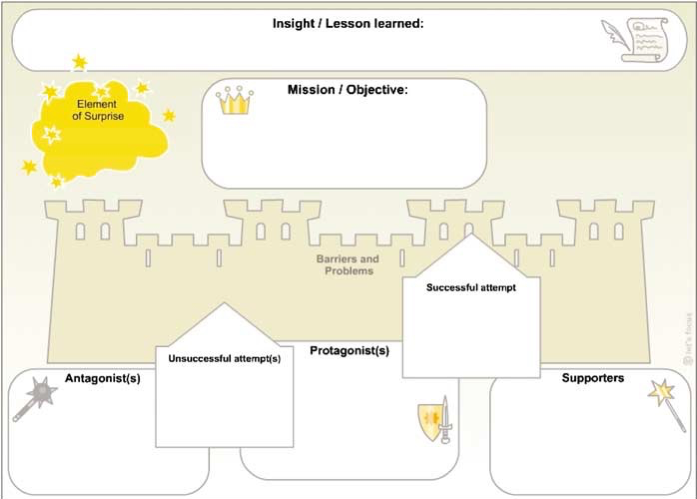
\includegraphics[width=0.75\linewidth]{visual-metaphor.jpg}}
	\caption{Example of a visual metaphor.}
	\label{fig:visual-metaphor}
\end{figure}

As you can see in the figure, the visualization is completely adapted to the specific case of the topic. In this way, it is very difficult to create a generic metaphor, which can be used for different topics. As our tool should be usable for different topics, the technique of visual metaphors is not suitable for the needs of our tool.


% --------------------------
% ----- KNOWLEDGE MAPS -----
% --------------------------
\section{Knowledge Maps}
According to \cite{knowledgemapsbalaid}, \textit{knowledge maps} is an umbrella term for tools and techniques like mind maps. \cite{knowledgemapsodonnell} defined the concept as follows:

\begin{quote}
``Knowledge maps are node-link representations in which ideas are located in nodes and connected to other related ideas through a series of labeled links.'' \hfill 
\end{quote}

This way of representing information has for example a positive impact on students. The paper of \cite{knowledgemapsodonnell} teaches us that students using knowledge maps are better in remembering the main ideas of the subject in comparison to the ones that study from the text without the visualization. As GuideaMaps's purpose is more focused on representing large amounts of knowledge in an easy to grasp way, remembering the content is less important. However, the node-link representation with the main idea in the center also showed to be useful for this purpose, as illustrated by the popularity of mind maps.\\

Next to mind maps, concept maps is a second technique included under the umbrella of knowledge maps. Concept maps are in some sense similar to mind maps but they do have some different characteristics. First, the purpose of a mind map is to associate ideas, topics or things, while concept maps illustrate relations between concepts. Further, the structure of a concept map is mostly hierarchical and visualized like a tree. On the other hand, mind maps sometimes have a radial layout and not hierarchical. \citep{davies} \\

Hence, we can state that GuideaMaps makes use of a knowledge map visualization and more specifically some kind of combination of mind maps and concept maps.



